\documentclass[varwidth=true, border=2pt]{standalone}
\usepackage{tikz}
\usetikzlibrary{positioning, calc}

\begin{document}
  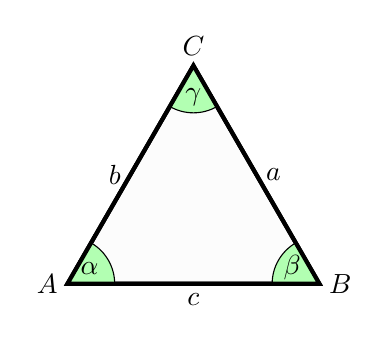
\begin{tikzpicture}[scale=0.8]
    % draw the background
    \draw [line width=1.5pt, fill=gray!2] (0,0) -- (60:4) -- (4,0) -- cycle;

    \coordinate[label=left:$A$]  (A) at (0,0);
    \coordinate[label=right:$B$] (B) at (4,0);
    \coordinate[label=above:$C$] (C) at (2,3.464);

    \coordinate[label=below:$c$](c) at ($ (A)!.5!(B) $);
    \coordinate[label=left:$b$] (b) at ($ (A)!.5!(C) $);
    \coordinate[label=right:$a$](a) at ($ (B)!.5!(C) $);

    % angle alpha
    \draw[fill=green!30] (0,0) -- (0:0.75cm) arc (0:60:.75cm);
    \draw (0.35cm,0.25cm) node {$\alpha$};

    % angle beta
    \begin{scope}[shift={(4cm,0cm)}]
        \draw[fill=green!30] (0,0) -- (-180:0.75cm) arc (180:120:0.75cm);
        \draw (150:0.5cm) node {$\beta$};
    \end{scope}

    % angle gamma
    \begin{scope}[shift={(60:4)}]
        \draw[fill=green!30] (0,0) -- (-120:.75cm) arc (-120:-60:.75cm);
        \draw (-90:0.5cm) node {$\gamma$};
    \end{scope}

    % the triangle
    \draw [line width=1.5pt] (A) -- (B) -- (C) -- cycle;
  \end{tikzpicture}
\end{document}